% Copyright 2019 by Saeed Taghavi
%
% This file may be distributed and/or modified
%
% 1. under the LaTeX Project Public License and/or
% 2. under the GNU Public License.
%
% See the file doc/licenses/LICENSE for more details.

\documentclass{beamer}

% Setup appearance:

\usetheme{Darmstadt}
\usefonttheme[onlylarge]{structurebold}
\setbeamerfont*{frametitle}{size=\normalsize,series=\bfseries}
\setbeamertemplate{navigation symbols}{}


% Standard packages

\usepackage[english]{babel}
\usepackage[latin1]{inputenc}
\usepackage{times}
\usepackage[T1]{fontenc}


% Setup TikZ

\usepackage{tikz}
\usetikzlibrary{arrows}
\tikzstyle{block}=[draw opacity=0.7,line width=1.4cm]


% Author, Title, etc.

\title[Short title] 
{%
Phase-Dependent Suppression of Neuronal Oscillations
%
}

\author[Taghavi, Valizadeh]
{
  \textcolor{blue!50!black}{Saeed~Taghavi\inst{1}} \and
  Alireza~Valizadeh\inst{1,2}
}

\institute[IASBS and others]
{
  \inst{1}%
  IASBS, Zanjan, Iran
  \and
  \vskip-2mm
  \inst{2}%
  IPM, Tehran, Iran
}

\date[neurophysics 2020]
{Conference on Neuroscience \\ and Physics of Neuronal Systems \\ 19 and 20 February 2020
\\
}





% The main document

\begin{document}

\begin{frame}
  \titlepage
\end{frame}

\begin{frame}{Outline}
  \tableofcontents
\end{frame}

%inja

\headerbox{Intruduction}{name=introduction,column=0, span=2}{
\large{
While synchronized oscillations within and between brain areas facilitate normal brain processing, excess synchrony usually is accompanied by a brain disease. A prominent example is the amplified persistent beta-frequency ($\sim$ 20 Hz) oscillations recorded from the cortex and subthalamic nucleus of Parkinsonian brains \cite{asllani2018minimally, holt2019phase}. Deep brain stimulation (DBS) is known to be an effective treatment for a variety of neurological disorders, including Parkinson's disease and essential tremor (ET). A common procedure is to impose a train of pulses with constant frequency via electrodes implanted into the brain. New 'closed-loop' approach involves delivering stimulation according to the ongoing brain activity and could improve in terms of efficiency and reduce side effects. The success of closed-loop DBS depends on the design of a stimulation strategy that minimizes oscillations in neural activity associated with symptoms \cite{weerasinghe2019predicting}. An important step to this end is to construct a mathematical model, which can describe how the brain oscillations should change when stimulation is applied at a particular state of the system.  
}
\vspace{0.4em}
}

\headerbox{DBS strategies}{name=introplot,column=2, span=1}{
\vspace*{-0.17cm}

\center{
\includegraphics[width=.75\linewidth]{fig/dbs_strategy.png} 
}

}

\section{Update rule}
the update rule which I have used is:
\begin{equation}
\theta_i^{t_n+1} = \theta_i^{t_n} + dt (\omega_i + K r^{t_n} \sin(\psi^{t_n} - \theta_i^{t_n})) + \alpha \mathcal{N} (0,\sqrt{dt}), \quad i \in \{ 1,...,N_{Osci} \}
\end{equation}
Initial phases produced with a random uniform distibution in $[0,2\pi]$.
\\
Natural frequencies ($\omega_i$) are all set to be $2\pi$.
\\
$\alpha=0.5$
\\
$r$ and $\psi$ are respectively the real and the imaginary part of the order parameter at each time step.
\\
And I have changed the coupling constant $K$ to be $1,2$ and $5$; stated at each plot.

\begin{figure}
	\includegraphics[width=.8\textwidth]{1.png}
	\caption{$K=1$}
\end{figure}

\begin{figure}
\includegraphics[width=.8\textwidth]{2.png}
\caption{$K=1$}
\end{figure}

\begin{figure}
\includegraphics[width=.8\textwidth]{3.png}
\caption{$K=1$}
\end{figure}

\begin{figure}
	\includegraphics[width=.8\textwidth]{11.png}
	\caption{$K=2$}
\end{figure}

\begin{figure}
\includegraphics[width=.8\textwidth]{12.png}
\caption{$K=2$}
\end{figure}

\begin{figure}
\includegraphics[width=.8\textwidth]{13.png}
\caption{$K=2$}
\end{figure}



\begin{figure}[hb!]
	\includegraphics[width=.8\textwidth]{21.png}
	\caption{$K=5$}
\end{figure}

\begin{figure}[hb!]
\includegraphics[width=.8\textwidth]{22.png}
\caption{$K=5$}
\end{figure}

\begin{figure}[hb!]
\includegraphics[width=.8\textwidth]{23.png}
\caption{$K=5$}
\end{figure}


%produced with a random normal distibution with Mean$=1$ and StandardDeviation=
%
%\begin{figure}[ht]
%  \centering
%  \begin{minipage}{.7\linewidth}
%    \begin{algorithm}[H]
%      \SetAlgoLined
%      \KwData{this text}
%      \KwResult{how to write algorithm with \LaTeX2e }
%      initialization\;
%      \While{not at end of this document}{
%        read current\;
%        \eIf{understand}{
%          go to next section\;
%          current section becomes this one\;
%        }{
%          go back to the beginning of current section\;
%        }
%      }
%      \caption{How to write algorithms}
%    \end{algorithm}
%  \end{minipage}
%\end{figure}

\headerbox{Conclusion}{name=subtopic1,column=2,below=results1,span=1}{
\large{
The amplitude of collective oscillations could be modulated depending on the specific phase at which the stimulation is applied. 

Also, we could predict the $good \ time$ for applying stimulation to get the maximum reduction in the oscillation amplitude based on the phase response curve (PRC) of oscillators.
}
\\

\\

\vspace*{1.6cm}
}


\headerbox{Discussion}{name=subtopic3,column=0,below=results1,span=2}{
%\vspace{0.3cm}
\begin{multicols}{2}
\large{

\center{
%\vspace*{-.5cm}
\includegraphics[width=0.8\linewidth]{fig/deltaR-Z} 
}

\center{
%\vspace*{-.5cm}
\includegraphics[width=0.7\linewidth]{fig/multi_stim} 
}


Applying multiple stimulations 

}
\end{multicols}

%\vspace{2cm} %remove this, only added for spacing
}


\section*{Conclusion}

\begin{frame}
  \frametitle<presentation>{Summary}

  \begin{itemize}
  \item
    Finding optimal pp-partitions is \alert{intractable}. 
  \item
    It is even intractable to find a pp-partition when \alert{just two 
      noncontiguous  blocks are known to suffice}.
  \item
    For perfect \alert{path} phylogenies, optimal partitions can be
    computed \alert{in polynomial time}.
  \end{itemize}

   \uncover<2>{
     \begin{columns}[t]
    \column{.5\textwidth}
    \begin{block}{}
    \begin{center}
      Thank you for listening!
      \\
      Any Questions?
    \end{center}

    \end{block}
    \end{columns}  
%  \begin{block}{}
%  {
%  \begin{center}
%
%  
%  \end{center}
%  }
%  \end{block}   
   } 
\end{frame}



\appendix

\section*{Appendix}

\begin{frame}[label=algorithm]{The algorithm in action.}{Computation of
    the partial order.}
  \begin{columns}[t]
    \column{.4\textwidth}
    \begin{exampleblock}{Genotype matrix}
      $G\colon$
      \begin{tabular}{ccccc}
        A & B & C & D & E \\\hline
        2 & 2 & 2 & 2 & 2 \\
        0 & 1 & 2 & 1 & 0 \\
        1 & 0 & 0 & 1 & 2 \\
        0 & 2 & 2 & 0 & 0
      \end{tabular}
    \end{exampleblock}
    \column{.6\textwidth}
    \begin{exampleblock}{Partial order}
      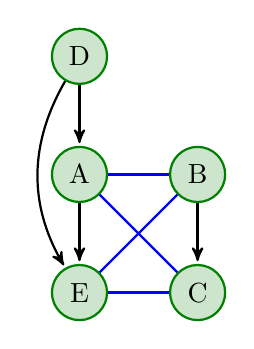
\begin{tikzpicture}[node distance=15mm]
        \tikzstyle{every node}=
        [%
          fill=green!50!black!20,%
          draw=green!50!black,%
          minimum size=7mm,%
          circle,%
          thick%
        ]

        \node (A) {A};
        \node (B) [right of=A] {B};
        \node (C) [below of=B] {C};
        \node (D) [above of=A] {D};
        \node (E) [below of=A] {E};

        \path [thick,shorten >=1pt,-stealth'] (A) edge (E)
                         (B) edge (C)
                         (D) edge (A)
                             edge[bend right] (E);

        \uncover<2>{
        \path [-,blue,thick](A) edge (B)
                                edge (C)  
                            (B) edge (E)
                            (C) edge (E);}
      \end{tikzpicture}

      Partial order: \tikz[baseline] \draw[thick,-stealth'] (0pt,.5ex)
      -- (5mm,.5ex); 

      \uncover<2>{\textcolor{blue}{Compatible as children of root:
          \tikz[baseline] \draw[thick] (0pt,.5ex) -- (5mm,.5ex);}} 
    \end{exampleblock}
  \end{columns}  
\end{frame}

\begin{frame}{The algorithm in action.}{The matching in the special graph.}
  \begin{columns}[t]
    \column{.3\textwidth}
    \begin{exampleblock}{Partial order}
      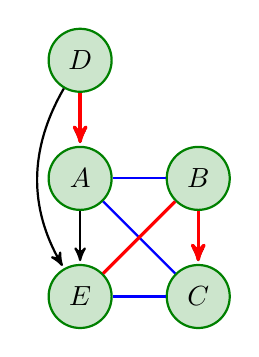
\begin{tikzpicture}[node distance=15mm]
        \tikzstyle{every node}=%
        [%
          fill=green!50!black!20,%
          draw=green!50!black,%
          minimum size=8mm,%
          circle,%
          thick%
        ]

        \node (A)              {$A$};
        \node (B) [right of=A] {$B$};
        \node (C) [below of=B] {$C$};
        \node (D) [above of=A] {$D$};
        \node (E) [below of=A] {$E$};

        \path [thick,shorten >=1pt,-stealth'] (A) edge (E)
                         (B) edge (C)
                         (D) edge (A)
                             edge[bend right] (E);

        \path [-,blue,thick](A) edge (B)
                                edge (C)  
                            (B) edge (E)
                            (C) edge (E);

        \only<3->
        {
          \path[very thick,shorten >=1pt,-stealth',red] (D) edge (A) (B) edge (C);
          \path [-,red,very thick](E) edge (B);
        }
      \end{tikzpicture}
    \end{exampleblock}
    \column{.7\textwidth}
    \begin{exampleblock}{Matching graph}
      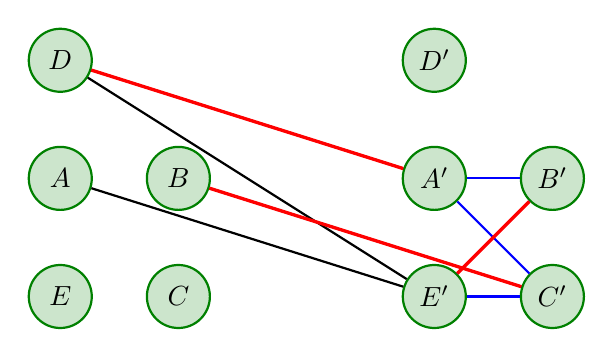
\begin{tikzpicture}[node distance=15mm]
        \tikzstyle{every node}=%
        [%
          fill=green!50!black!20,%
          draw=green!50!black,%
          minimum size=8mm,%
          circle,%
          thick,%
          inner sep=0pt%
        ]

        \node (A)              {$A$};
        \node (B) [right of=A] {$B$};
        \node (C) [below of=B] {$C$};
        \node (D) [above of=A] {$D$};
        \node (E) [below of=A] {$E$};

        \begin{scope}[xshift=4.75cm]
          \node (A')               {$A'$};
          \node (B') [right of=A'] {$B'$};
          \node (C') [below of=B'] {$C'$};
          \node (D') [above of=A'] {$D'$};
          \node (E') [below of=A'] {$E'$};
        \end{scope}
        
        \path [thick]    (A) edge (E')
                         (B) edge (C')
                         (D) edge (A')
                             edge (E');

        \path [blue,thick](A') edge (B')
                               edge (C')  
                          (B') edge (E')
                          (C') edge (E');

        \only<2->
        {
          \path[very thick,red] (D) edge (A')
                           (B) edge (C')
                           (B') edge (E');
        }
      \end{tikzpicture}
    \end{exampleblock}
  \end{columns}

  \medskip
  \uncover<2->{A \alert{maximal matching} in the matching graph
    \uncover<3>{induces\\ \alert{perfect path phylogenies}.}}

  \hfill\hyperlink{return}{\beamerreturnbutton{Return}}
\end{frame}

\end{document}


